\documentclass[a4paper,14pt]{article}

%%% Работа с русским языком
\usepackage{cmap}					% поиск в PDF
\usepackage{mathtext} 				% русские буквы в формулах
\usepackage[T2A]{fontenc}			% кодировка
\usepackage[utf8]{inputenc}			% кодировка исходного текста
\usepackage[english,russian]{babel}	% локализация и переносы
\usepackage{indentfirst}
\frenchspacing

\renewcommand{\epsilon}{\ensuremath{\varepsilon}}
\renewcommand{\phi}{\ensuremath{\varphi}}
\renewcommand{\kappa}{\ensuremath{\varkappa}}
\renewcommand{\le}{\ensuremath{\leqslant}}
\renewcommand{\leq}{\ensuremath{\leqslant}}
\renewcommand{\ge}{\ensuremath{\geqslant}}
\renewcommand{\geq}{\ensuremath{\geqslant}}
\renewcommand{\emptyset}{\varnothing}

\newcommand{\bS}{\mathbf{S}}
\newcommand{\bF}{\mathbf{F}}
\newcommand{\bw}{\mathbf{w}}
\newcommand{\T}{^{\mathsf{T}}}

%%% Дополнительная работа с математикой
\usepackage{amsmath,amsfonts,amssymb,amsthm,mathtools} % AMS
\usepackage{icomma} % "Умная" запятая: $0,2$ --- число, $0, 2$ --- перечисление

%% Номера формул
%\mathtoolsset{showonlyrefs=true} % Показывать номера только у тех формул, на которые есть \eqref{} в тексте.
%\usepackage{leqno} % Нумереация формул слева

%% Свои команды
\DeclareMathOperator{\sgn}{\mathop{sgn}}

%% Перенос знаков в формулах (по Львовскому)
\newcommand*{\hm}[1]{#1\nobreak\discretionary{}
	{\hbox{$\mathsurround=0pt #1$}}{}}

%%% Работа с картинками
\usepackage{graphicx}  % Для вставки рисунков
\setlength\fboxsep{3pt} % Отступ рамки \fbox{} от рисунка
\setlength\fboxrule{1pt} % Толщина линий рамки \fbox{}
\usepackage{wrapfig} % Обтекание рисунков текстом

%%% Работа с таблицами
\usepackage{array,tabularx,tabulary,booktabs} % Дополнительная работа с таблицами
\usepackage{longtable}  % Длинные таблицы
\usepackage{multirow} % Слияние строк в таблице

%%% Теоремы
\theoremstyle{plain} % Это стиль по умолчанию, его можно не переопределять.
\newtheorem{theorem}{Теорема}[section]
\newtheorem{proposition}[theorem]{Утверждение}
\newtheorem{definition}{Определение}

\theoremstyle{definition} % "Определение"
\newtheorem{corollary}{Следствие}[theorem]
\newtheorem{problem}{Задача}[section]

\theoremstyle{remark} % "Примечание"
\newtheorem*{nonum}{Решение}

%%% Программирование
\usepackage{etoolbox} % логические операторы

%%% Страница
\usepackage{extsizes} % Возможность сделать 14-й шрифт
\usepackage{geometry} % Простой способ задавать поля
\geometry{top=25mm}
\geometry{bottom=35mm}
\geometry{left=35mm}
\geometry{right=20mm}
%
%\usepackage{fancyhdr} % Колонтитулы
% 	\pagestyle{fancy}
%\renewcommand{\headrulewidth}{0pt}  % Толщина линейки, отчеркивающей верхний колонтитул
% 	\lfoot{Нижний левый}
% 	\rfoot{Нижний правый}
% 	\rhead{Верхний правый}
% 	\chead{Верхний в центре}
% 	\lhead{Верхний левый}
%	\cfoot{Нижний в центре} % По умолчанию здесь номер страницы

\usepackage{setspace} % Интерлиньяж
%\onehalfspacing % Интерлиньяж 1.5
%\doublespacing % Интерлиньяж 2
%\singlespacing % Интерлиньяж 1

\usepackage{lastpage} % Узнать, сколько всего страниц в документе.

\usepackage{soul} % Модификаторы начертания

\usepackage{hyperref}
\usepackage[usenames,dvipsnames,svgnames,table,rgb]{xcolor}
\hypersetup{				% Гиперссылки
	unicode=true,           % русские буквы в раздела PDF
	pdftitle={Заголовок},   % Заголовок
	pdfauthor={Автор},      % Автор
	pdfsubject={Тема},      % Тема
	pdfcreator={Создатель}, % Создатель
	pdfproducer={Производитель}, % Производитель
	pdfkeywords={keyword1} {key2} {key3}, % Ключевые слова
	colorlinks=true,       	% false: ссылки в рамках; true: цветные ссылки
	linkcolor=red,          % внутренние ссылки
	citecolor=black,        % на библиографию
	filecolor=magenta,      % на файлы
	urlcolor=cyan           % на URL
}

\usepackage{csquotes} % Еще инструменты для ссылок

%\usepackage[style=authoryear,maxcitenames=2,backend=biber,sorting=nty]{biblatex}

\usepackage{multicol} % Несколько колонок

\usepackage{tikz} % Работа с графикой
\usepackage{pgfplots}
\usepackage{pgfplotstable}


\author{Владимиров Эдуард, группа Б05-928}
\title{\textbf{Отчёт о лабораторной работе №1}}
\date{\today}

\begin{document}
	\maketitle
	Каждый отчет в отдельной подпапке помещается в папку "chapters".
	Данный отчёт выступает в качестве шаблона. В общем файле проекта "main.tex" добавьте свой отчет по аналогии с данным.
	
	\section{Введение}
	Цель лабораторной работы заключается в прогнозировании временного ряда на короткий промежуток времени с помощью \textbf{ARIMA}.
	Для достижения наилучшего прогноза используется выбор параметров модели. Эксперимент проводится на показаниях акселерометра c частотой 500 Гц.
	
	\section{Постановка задачи}
	Пусть значения многомерного временного ряда  
	\[ \bS(t) = [S_x(t), S_y(t), S_z(t), S_{acc}(t)] \T \]
	доступны в моменты времени $t = 1, 2, \ldots, n$. Необходимо предсказать значения временного ряда в моменты времени $n+1, \ldots, n+N$.  
	
	Для вычисления будущих значений временного ряда требуется определить функциональную зависимость, отражающую связь между прошлыми значениями $\bS(t)$ и будущими. Общий вид модели прогнозирования таков (более подробно о ней будет рассказано в разделе \ref{model_descr}. \nameref{model_descr}):
	\begin{equation*}
		\bS(t) = \bF(p, d, q, \bw, \bS(t-1), \ldots, \bS(1)) + \boldsymbol{\epsilon}_t.
	\end{equation*}
	где $p, d, q $ ~--- гиперпараметры модели $\bF$, о значении которых будет сказано позже.
	
	В качестве критерия качества модели выступает информационный критерий Шварца:
	\begin{equation*}
		\mathcal{Q} = \ln s^2 + \dfrac{(p + q) \ln m}{m}, \quad s^2 = \frac1m \sum\limits_{i=1}^m ||\boldsymbol{\epsilon}_t||^2,
	\end{equation*}
	где $m$ ~--- размер обучающей выборки. Функция потерь данной модели, по которой настраиваются параметры $w$ ~--- обычный MSE.
	
	\section{Модель} \label{model_descr}
	\begin{definition} 
		Временной ряд $\bS(t)$ удовлетворяет модели $ARMA(p, q)$, если
		\begin{equation*}
			\begin{split}
				\bS(t) = \mu &+ \phi_1 \bS(t-1) + \phi_2 \bS(t-2) + \ldots + \phi_p \bS(t-p) + \\ &+ \epsilon_t + \theta_1 \epsilon_{t-1} + 
				\theta_2 \epsilon_{t-2} + \ldots + \theta_q \epsilon_{t-q},
			\end{split}
		\end{equation*}
		где $\epsilon_t \sim \mathcal{N}(0, \sigma^2), \quad \mathsf{E}\epsilon_t\epsilon_s = 0 \text{ для } t \neq s.$
	\end{definition}
	
	Для удобства представления различных моделей часто используется
	(формальный) лаговый оператор $L$:
		\[ L(\bS(t)) = \bS(t-1)\]
	Далее
		\[ L^k(\bS(t)) = \bS(t-k) \]
	и формально положим $L^0(\bS(t)) = \bS(t).$
	
	\begin{definition}
		Временной ряд $\bS(t)$ удовлетворяет модели $ARIMA(p, d, q)$, если временной ряд разностей порядка $d$ $(1 - L)^d \bS(t)$ удовлетворяет модели $ARMA(p, q)$
	\end{definition}
	
	\section{Вычислительный эксперимент и анализ ошибки}
	Данные ~--- это показания трёхосевого акселерометра с частотой 500 Гц и длительностью использования 30 секунд (итого 15000 записей).  
	Также было вычислено само ускорение как $l2\text{-норма}$ вектора координатных ускорений. Полученный временной ряд был разбит на обучающую и тестовую части размера 12000 и 3000 соответственно.  
	
	Поскольку модель ARIMA из питоновского пакета stattools принимает только одномерные данные, и само обучение длится довольно долго, то предсказания были получены только для значений ускорения.
	
	\begin{figure}[bhtp]
		\centering
		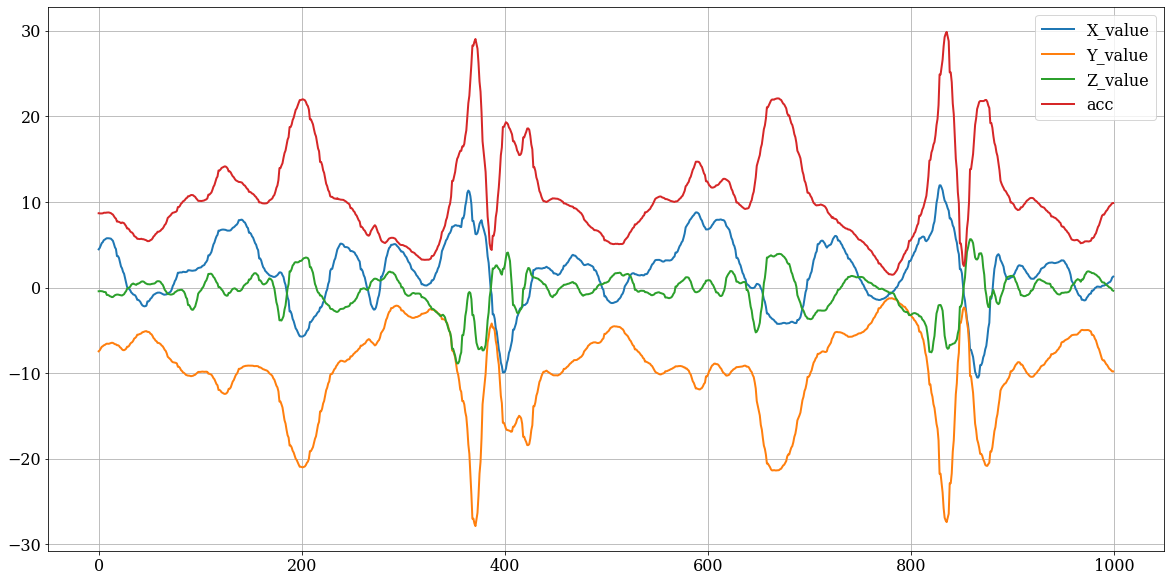
\includegraphics[width=\linewidth]{acc_data.png}
		\caption{Показания акселерометра + значение ускорения}
	\end{figure}
	
	Пайплайн обучения модели выглядит так:
	\begin{enumerate}
		\item[*] Исследование временного ряда на наличие выбросов. Применение преобразования Бокса-Кокса для $\lambda = 0$ с предварительным сдвигом (чтобы все значения были положительными)
		
		\item[*] Исследование графиков $ACF$ и $PACF$ для определения стационарности временного ряда. Использование сезонного дифференцирования. Повторное исследование уже новых графиков $ACF$ и $PACF$.
		
		\item[*] Проведение тестов $KPSS$ и $ADF$ для проверки стационарности ряда.
		
		\item[*] Выбор стартовых значений $p$ и $q$. Поиск оптимальных параметров модели $ARMA$ по сетке с минимальным информационным критерием Шварца
	\end{enumerate}

	\begin{figure}[bhtp]
		\centering
		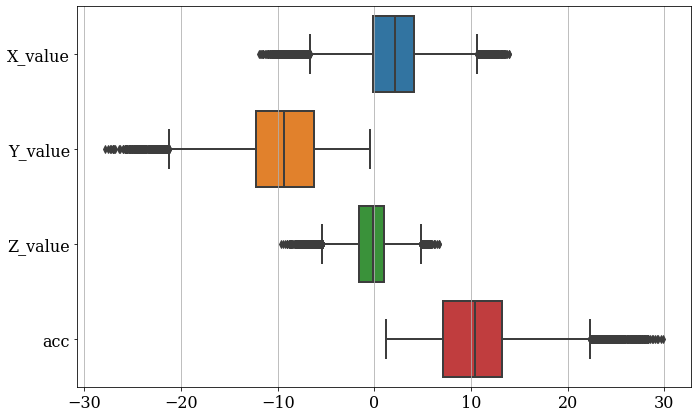
\includegraphics[width=\linewidth]{boxplot.png}
		\caption{Анализ временных рядов на наличие выбросов с помощью boxplot-ов}
	\end{figure}
	
	\begin{figure}[bhtp]
		\centering
		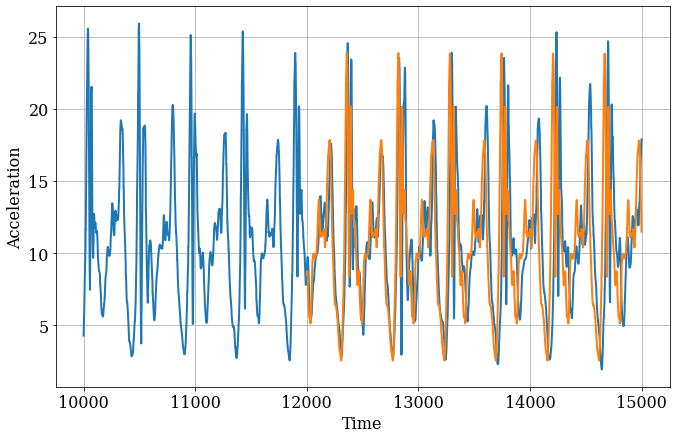
\includegraphics[width=\linewidth]{prediction_view.png}
		\caption{Полученные предсказания ускорения}
	\end{figure}

	\begin{figure}[bhtp]
		\centering
		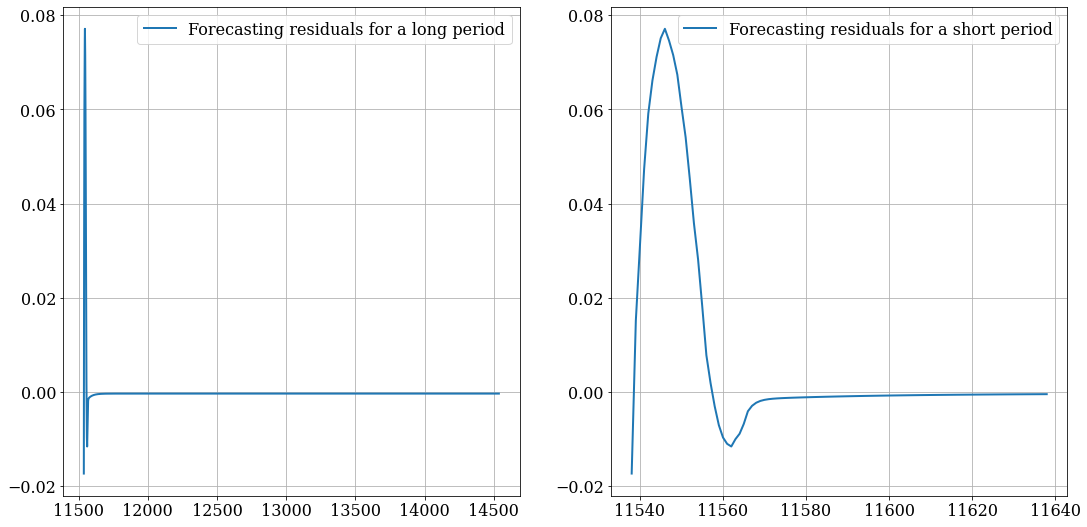
\includegraphics[width=\linewidth]{resid_pred.png}
		\caption{Предсказания стационарного дифф. ряда. Как видно из графика, модель ARMA даёт только краткосрочные “содержательные” прогнозы.}
	\end{figure}

	\renewcommand{\arraystretch}{1.5}
	\begin{table}[bhtp]
		\centering
		\caption{Значения различных функционалов качества}
		\begin{tabular}{|c|c|}
			\hline
			\textbf{Metric} & \multicolumn{1}{r|}{\textbf{Value}} \\ \hline
			MSE & $1.71 \pm 2.07$ \\ \hline
			MAE & $1.02 \pm 0.81$ \\ \hline
			MAPE & $0.13 \pm 0.00$ \\ \hline
		\end{tabular}
	\end{table}

	\section{Литература}
	Пользовался учебным пособием "Введение в анализ временных рядов", авторами которого являются Н.~В.~Артамонов, Е.~А.~Ивин, А.~Н.~Курбацкий, Д.~Фантаццини
\end{document}
